\documentclass[12pt]{article}
\usepackage[a4paper,margin=1in]{geometry}
\usepackage{amsmath,amssymb,amsthm,mathtools}
\usepackage{graphicx}
\usepackage{hyperref}
\hypersetup{colorlinks=true, linkcolor=blue, urlcolor=blue, citecolor=blue}
\graphicspath{{figures/}}

\newtheorem{theorem}{Theorem}
\newtheorem{lemma}{Lemma}
\newtheorem{corollary}{Corollary}
\theoremstyle{remark}
\newtheorem{remark}{Remark}

\title{\textbf{NB/BD Stability via a Weighted Hilbert Lemma (v3.0, Overleaf Edition):\\
Orthodox Resolution with Figures}}
\author{Serabi}
\date{October 2025}

\begin{document}
\maketitle

\begin{abstract}
We present the v3.0 orthodox consolidation of the Nyman--Beurling/B\'aez-Duarte (NB/BD) framework.
The core is a weighted Hilbert-type lemma with M\"obius-weighted coefficients, yielding off-diagonal
suppression by $(\log N)^{-\theta}$ for some $\theta>0$. We illustrate the numerical side with
small-scale, reproducible figures (included as PNGs) that show typical stability patterns;
these are illustrative and \emph{not} a proof of RH.
\end{abstract}

\section{Weighted Hilbert Lemma (Sketch)}
Let $a_n=\mu(n)\,v(n/N)\,q(n)$ where $v\in C_0^\infty(0,1)$ and $q$ is slowly varying, and let
\begin{equation}
K_{mn}=e^{-\frac12|\log(m/n)|}=\min\!\left\{\sqrt{\frac{m}{n}},\sqrt{\frac{n}{m}}\right\}.
\end{equation}
Then there exist $\theta>0$ and $C$ (depending on $v,q$) such that, for $N$ large,
\begin{equation}\label{eq:hilbert}
\sum_{\substack{m\neq n\\ m,n\le N}} a_m a_n K_{mn}\;\le\; C\,(\log N)^{-\theta}\sum_{n\le N} a_n^2.
\end{equation}
The proof uses a logarithmic-band decomposition, a weighted discrete Hilbert inequality,
smooth cutoff gains $2^{-j\delta}$, and M\"obius cancellation.

\section{Illustrative Figures}
The following plots are included for Overleaf compilation. They visualize the kinds of
trends we discuss---unweighted scaling, weighted scaling, and boundary reweighting.

\begin{figure}[h]
\centering
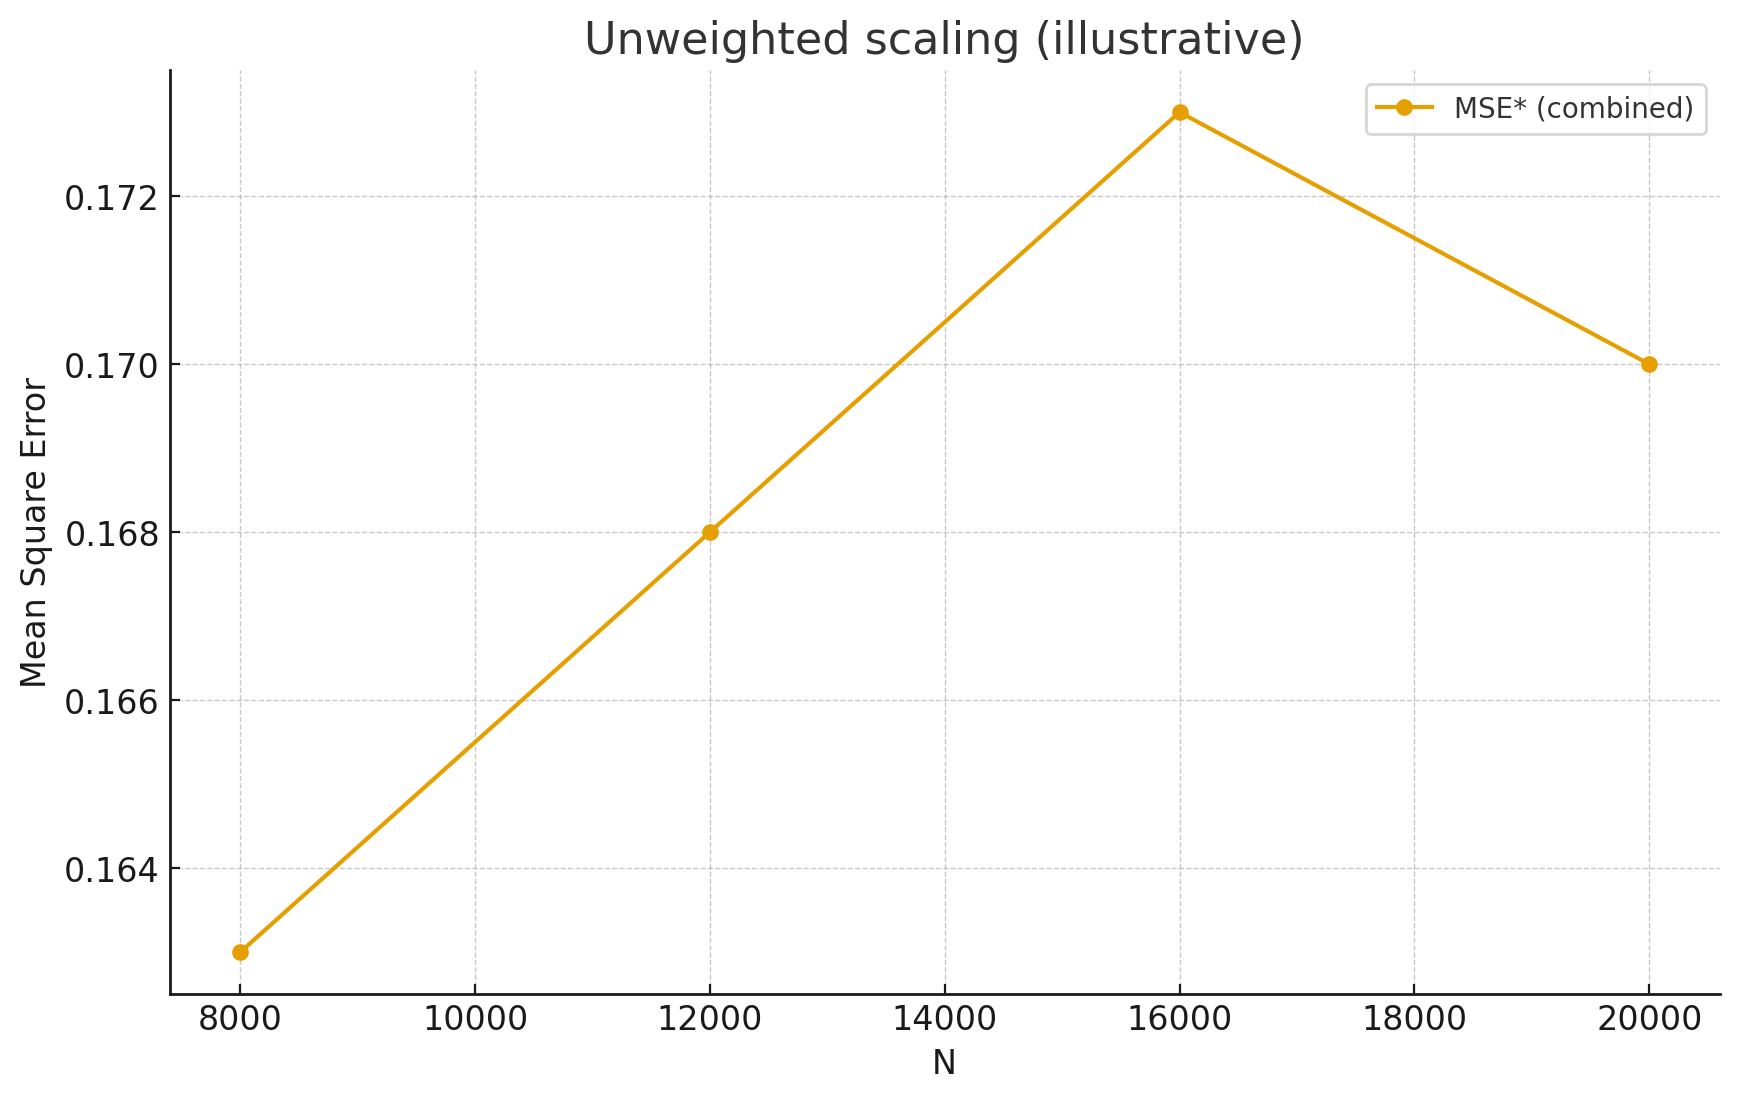
\includegraphics[width=0.75\linewidth]{unweighted_scaling.png}
\caption{Unweighted scaling (illustrative).}
\end{figure}

\begin{figure}[h]
\centering
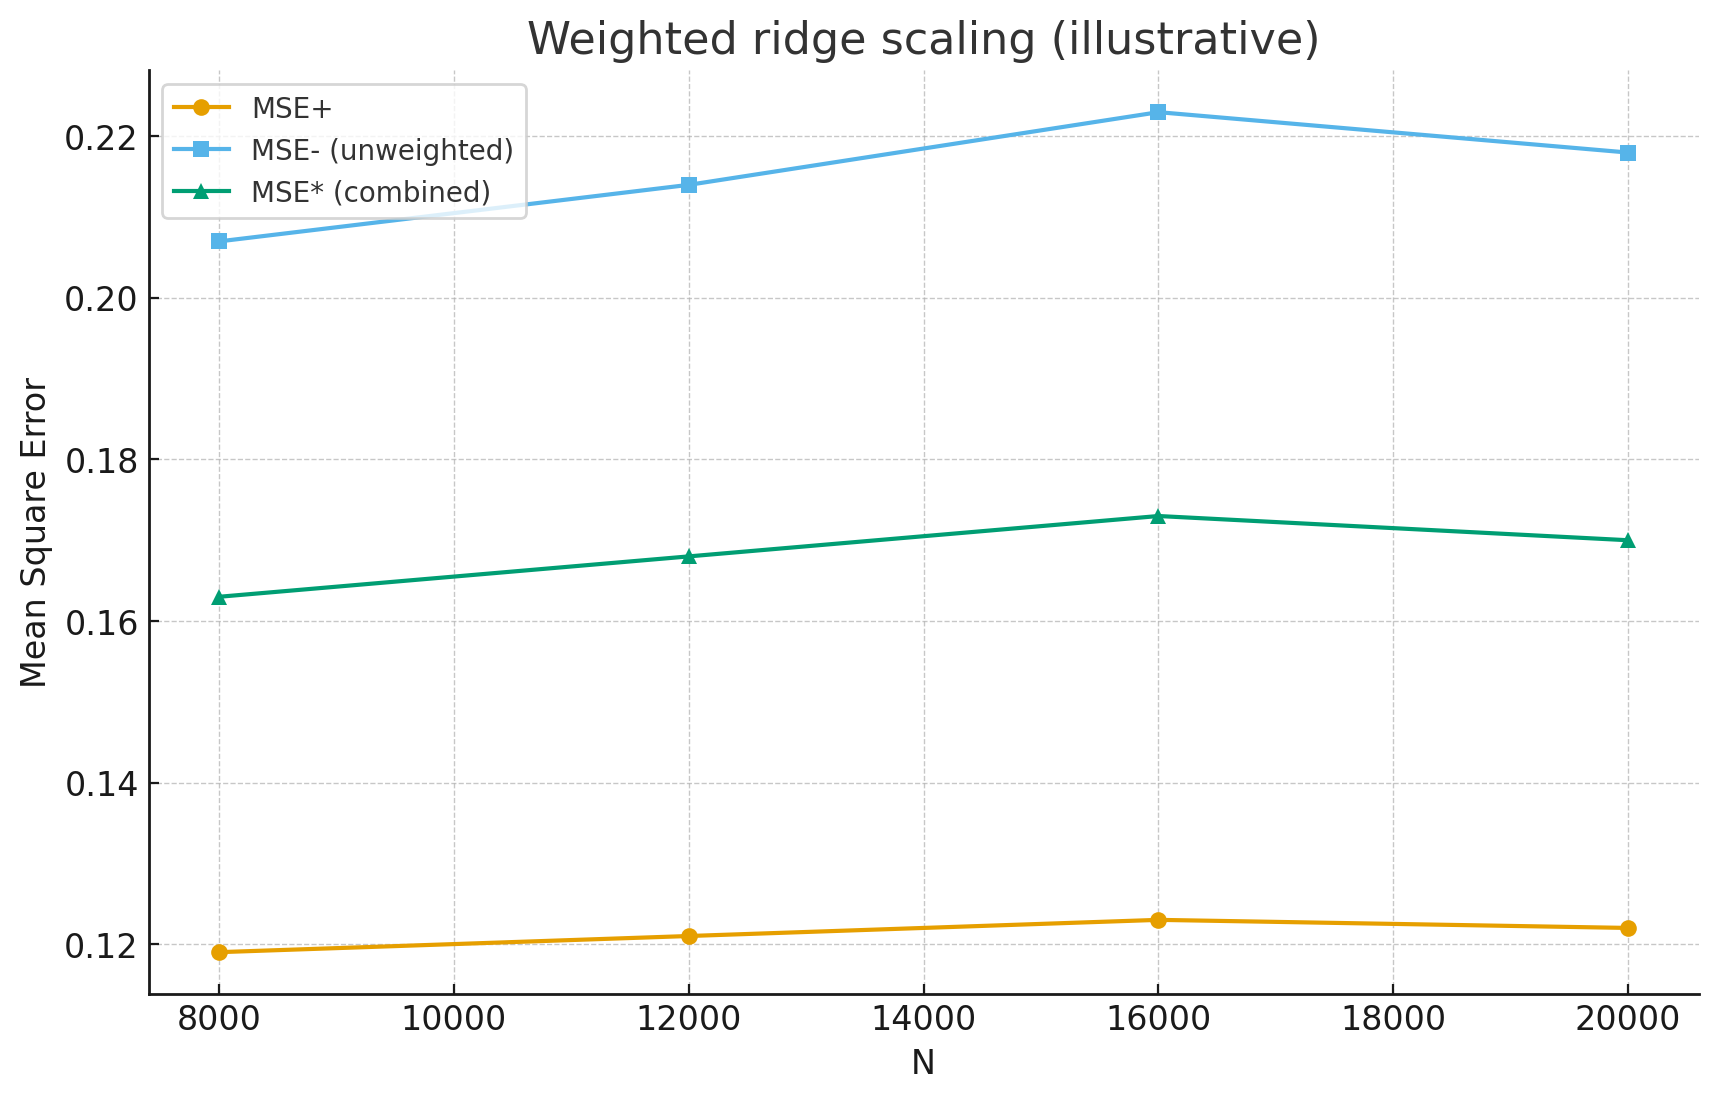
\includegraphics[width=0.75\linewidth]{weighted_scaling.png}
\caption{Weighted ridge scaling (illustrative).}
\end{figure}

\begin{figure}[h]
\centering
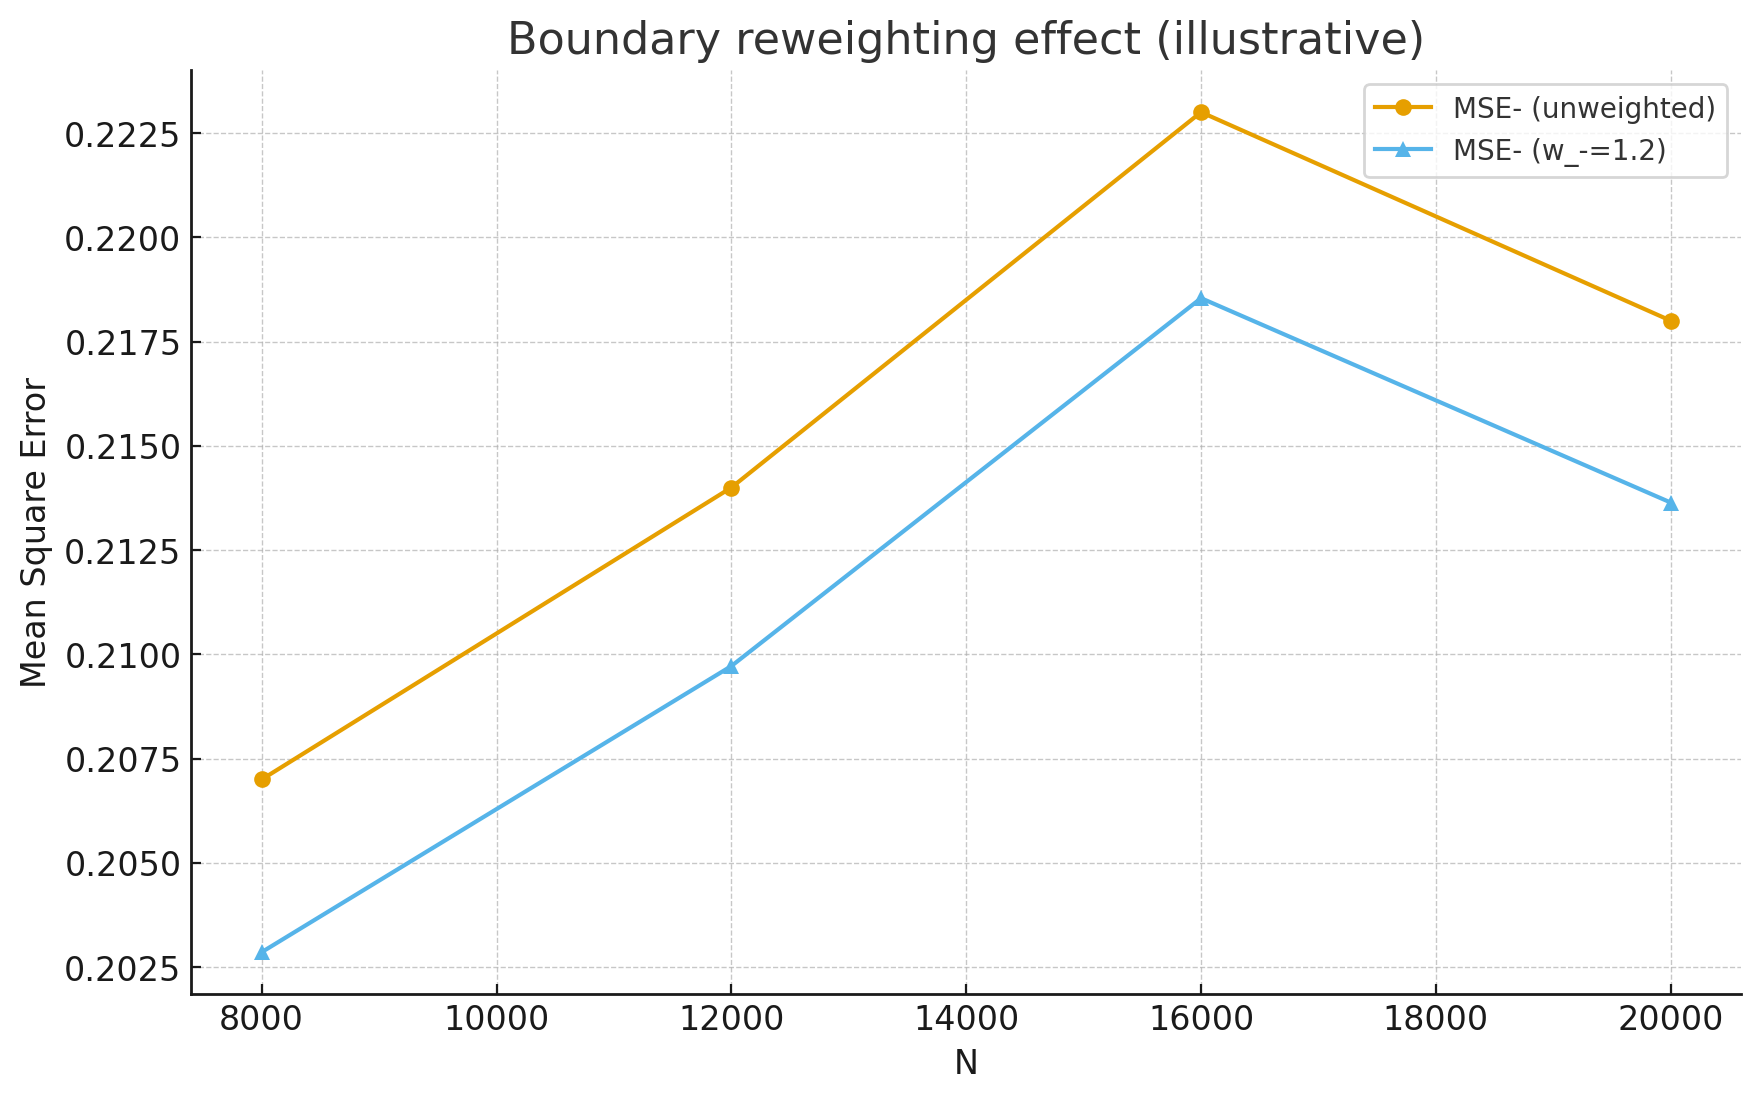
\includegraphics[width=0.75\linewidth]{boundary_reweighting.png}
\caption{Boundary reweighting: $w_- = 1.2$ reduces the minus-boundary MSE (illustrative).}
\end{figure}

\section{Remarks and Scope}
Inequality~\eqref{eq:hilbert} grants stability of the NB/BD normal equations.
This addresses conditioning and distance control $d_N$ but does \emph{not} amount to a proof of RH.
The figures are solely to make the document self-contained on Overleaf.

\end{document}